\chapter{Data Evaluation}\label{chap:de}
This chapter is a consequence of the conducted and normalized measurements performed using a single-antenna \acs{DUT} and a multi-antenna \acs{DUT}. Each test is run for many times in-order to assess the \acf{MU}. 

\section{Measurement Analysis}
This section is sub-divided into two other sections: first when the \acs{DUT} behaves as a transmitter and second when \acs{DUT} is a receiver. This sections also explains the reasons for using the fritz box as a companion device for \acs{PSD} measurement and for using some different spectrum analyzer settings from the settings mentioned by the standard.


\subsection{\acs{DUT} functions as transmitter}
The procedure for the \acf{OBW} measurement and \acf{PSD} are explained in detail in chapter \ref{chap:test}. Figure \ref{fig:nt} depicts the measurement when the \acs{DUT} acts like a transmitter and sends echo packets. The spectrum analyzer saves the traces so that we can measure the bandwidth and the \acf{PSD} of the signal from the \acs{DUT}. When using a golden device or fritz box (section \ref{sec:golden}) as a companion device, data is transmitted and not just \acs{ICMP} packets.


\begin{figure}[H]
\centering
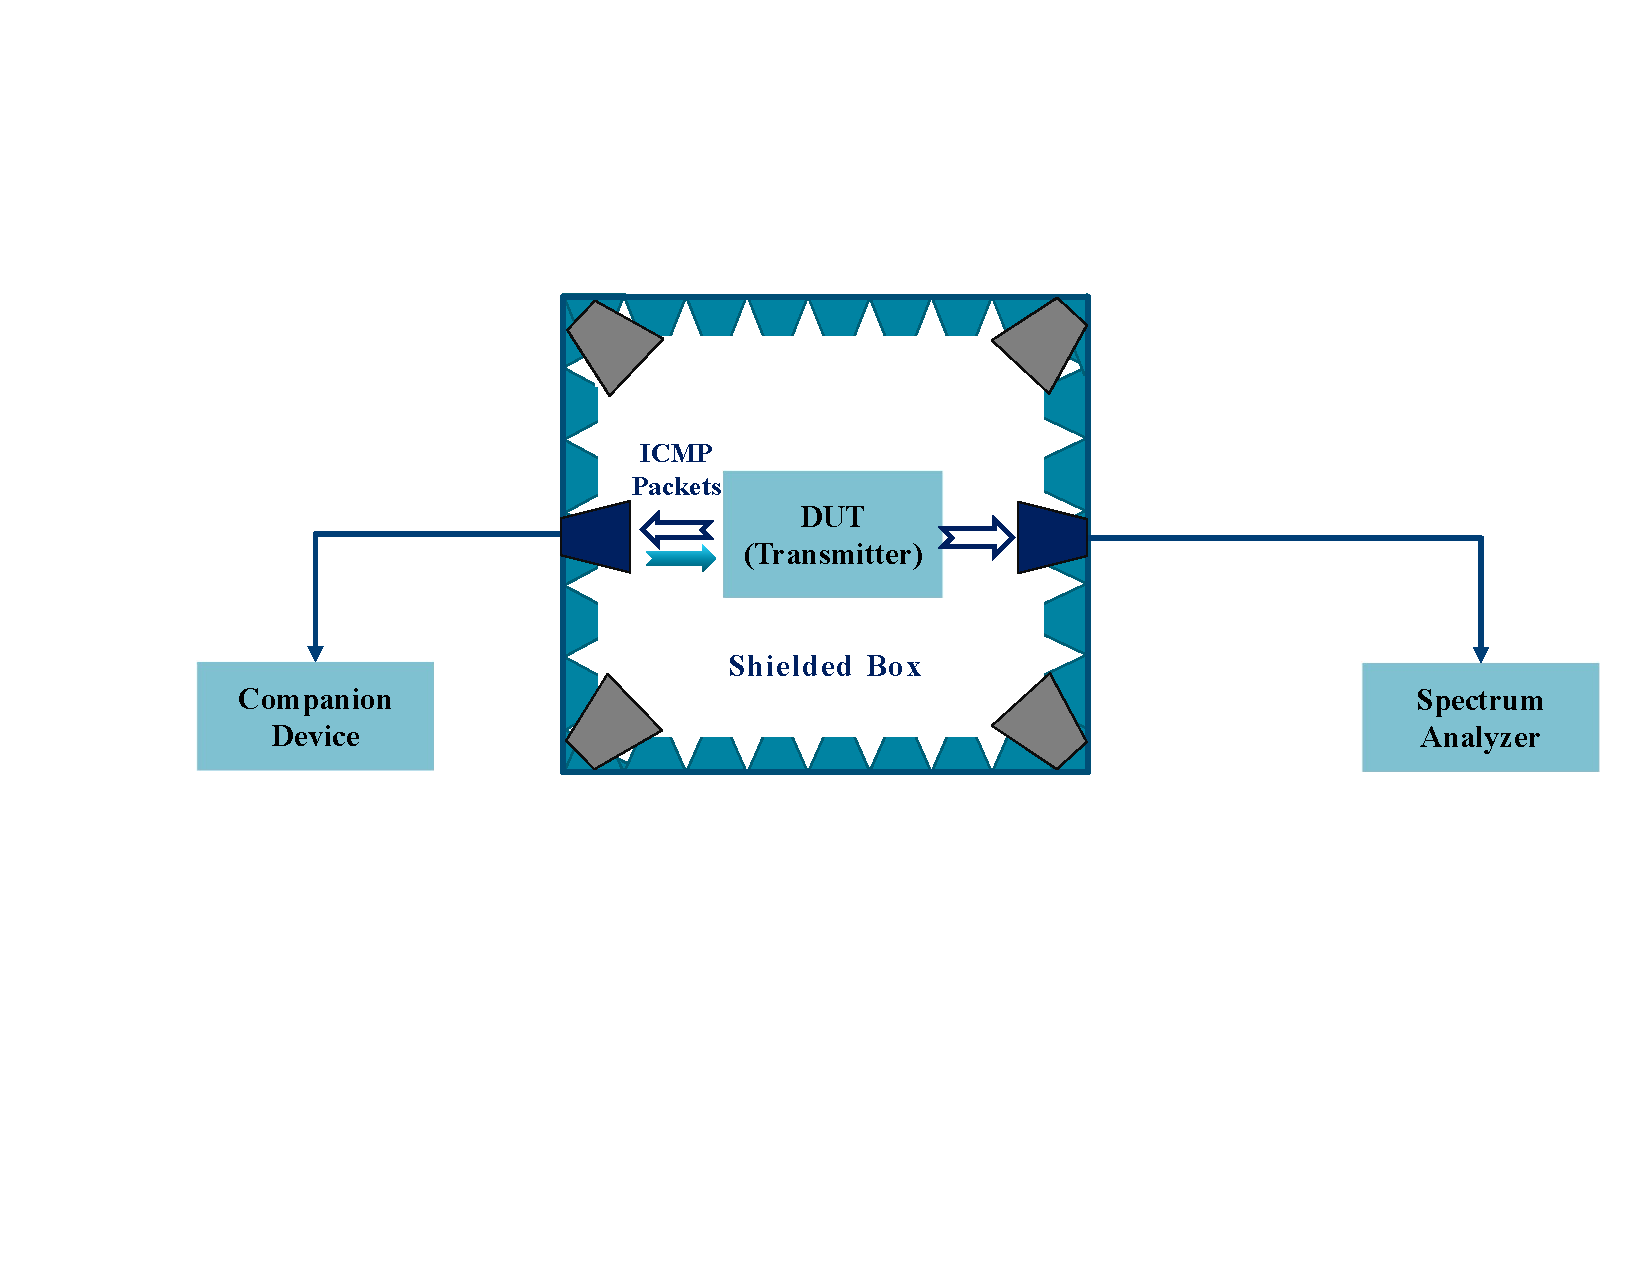
\includegraphics[scale = 0.46]{normalized_dut_transmitter.pdf}
\vspace{-0.5cm}
\caption{Normalized measurement when the \acs{DUT} functions as a transmitter}
\label{fig:nt} 
\end{figure}

Attenuation in the signal analyzer settings is kept to 10 dB and the pre-amplification is switched-off for conducted measurements because of the need of the signal to have a  high dynamic-range, i.e. to make sure that the power envelope is sufficiently above the noise floor of the analyser and to avoid the noise signals left and right from the power envelope being taken into account by this measurement. But, during radiated measurements, the pre-amplification is switched-on and the attenuation is brought down to 0 dB. This is because if the same conducted measurement settings are applied to radiated measurements, the dynamic-range and the noise floor of the signal is low which therefore increases the bandwidth of the signal (Figure \ref{fig:o}). 

\begin{figure}[H]
  \centering
  \subfigure[Bandwidth measurement with proper analyzer settings]{\includegraphics[width=0.49\textwidth]{OCBW_OTA_ATT0.png}} 
  \centering
  \subfigure[Low dynamic range of the system causing increase in bandwidth]{\includegraphics[width=0.49\textwidth]{{OCBW_OTA_ATT10.png}}} 
\caption{Increase in bandwidth of the signal due to low dynamic range}
\label{fig:o}
\end{figure}

The settings for the analyzer mentioned above also applies to \acf{PSD} measurement. In-addition to that, after running the \acs{PSD} measurement only for few times, there is a difference in the result every single time. This can be clearly seen from Figure \ref{fig:psdpsd}. The maximum value is 8.64 dBm and minimum is 7.12 dBm and hence there difference between the two is around 1 dBm which does not look very good. Therefore fritz box is used as a companion device for this measurement instead of the connectivity tester.
\begin{figure}[H]
\centering
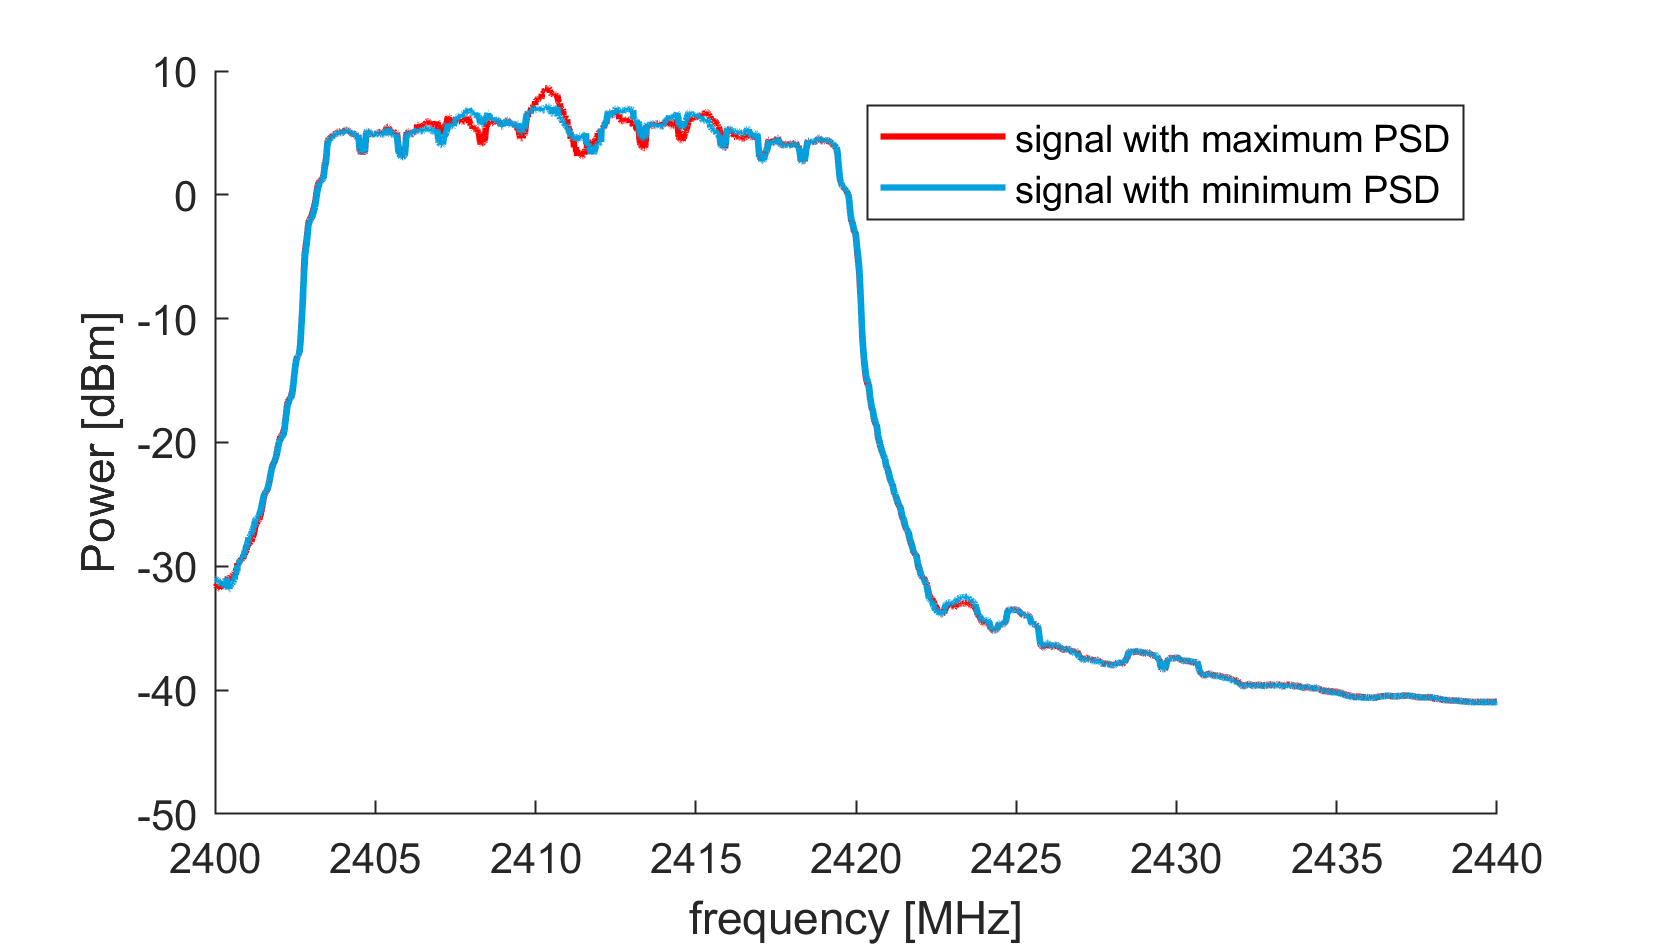
\includegraphics[scale = 0.75]{PSD_trace_differnce.png}
\caption{\acf{MU} in the \acs{PSD} measurement caused due to low duty cycle of the signal}
\label{fig:psdpsd} 
\end{figure}



\subsection{\acs{DUT} functions as receiver}
Figure \ref{fig:nr} pictures the \acs{DUT} as a receiver. This is achieved by using \acf{PER} measurement (section \ref{sec:rxmeas}).

\begin{figure}[H]
\centering
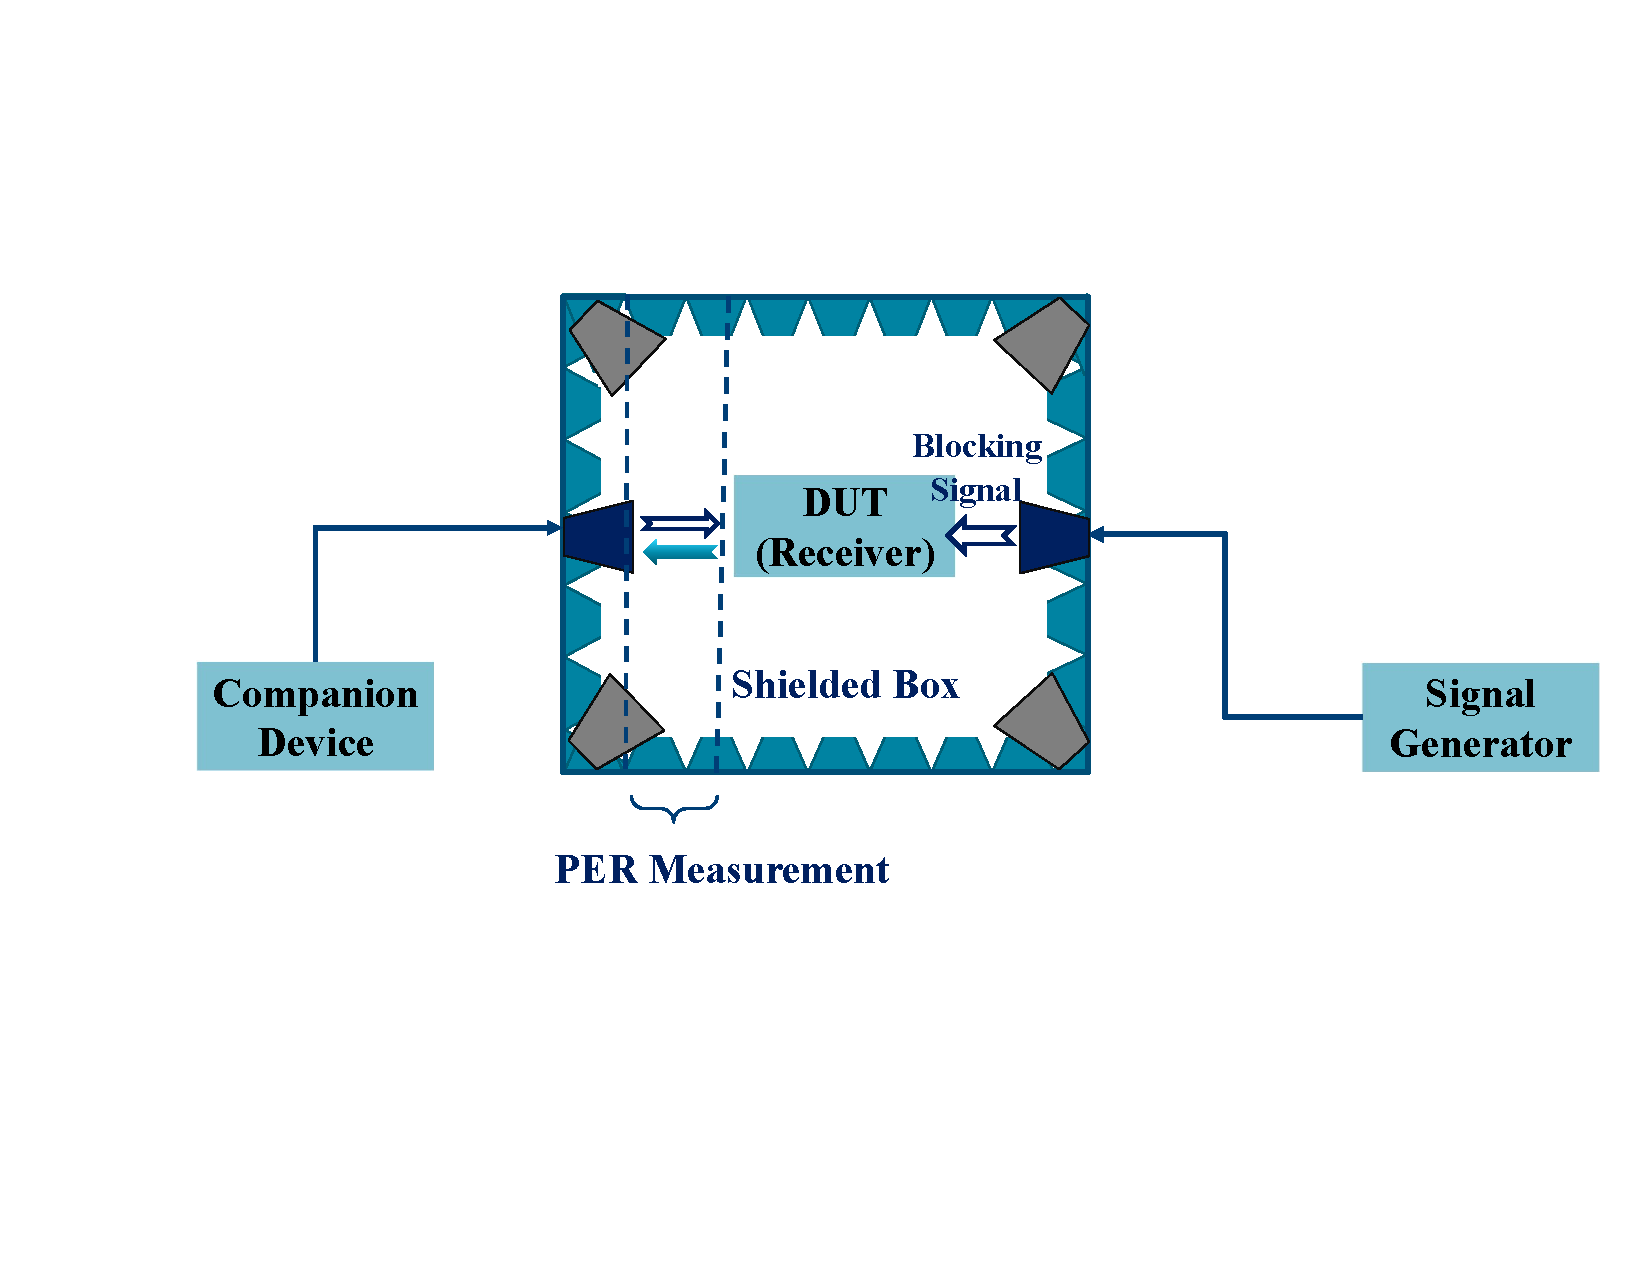
\includegraphics[scale = 0.46]{normalized_dut_receiver.pdf}
\vspace{-1.1cm}
\caption{Normalized measurement when the \acs{DUT} functions as a receiver}
\label{fig:nr} 
\end{figure}

The spectrum analyzer shows the DUT signal and the blocking signal. It can be seen that the signal from the blocker is not very far from the in-band frequency of the \acs{DUT}.
\begin{figure}[H]
\centering
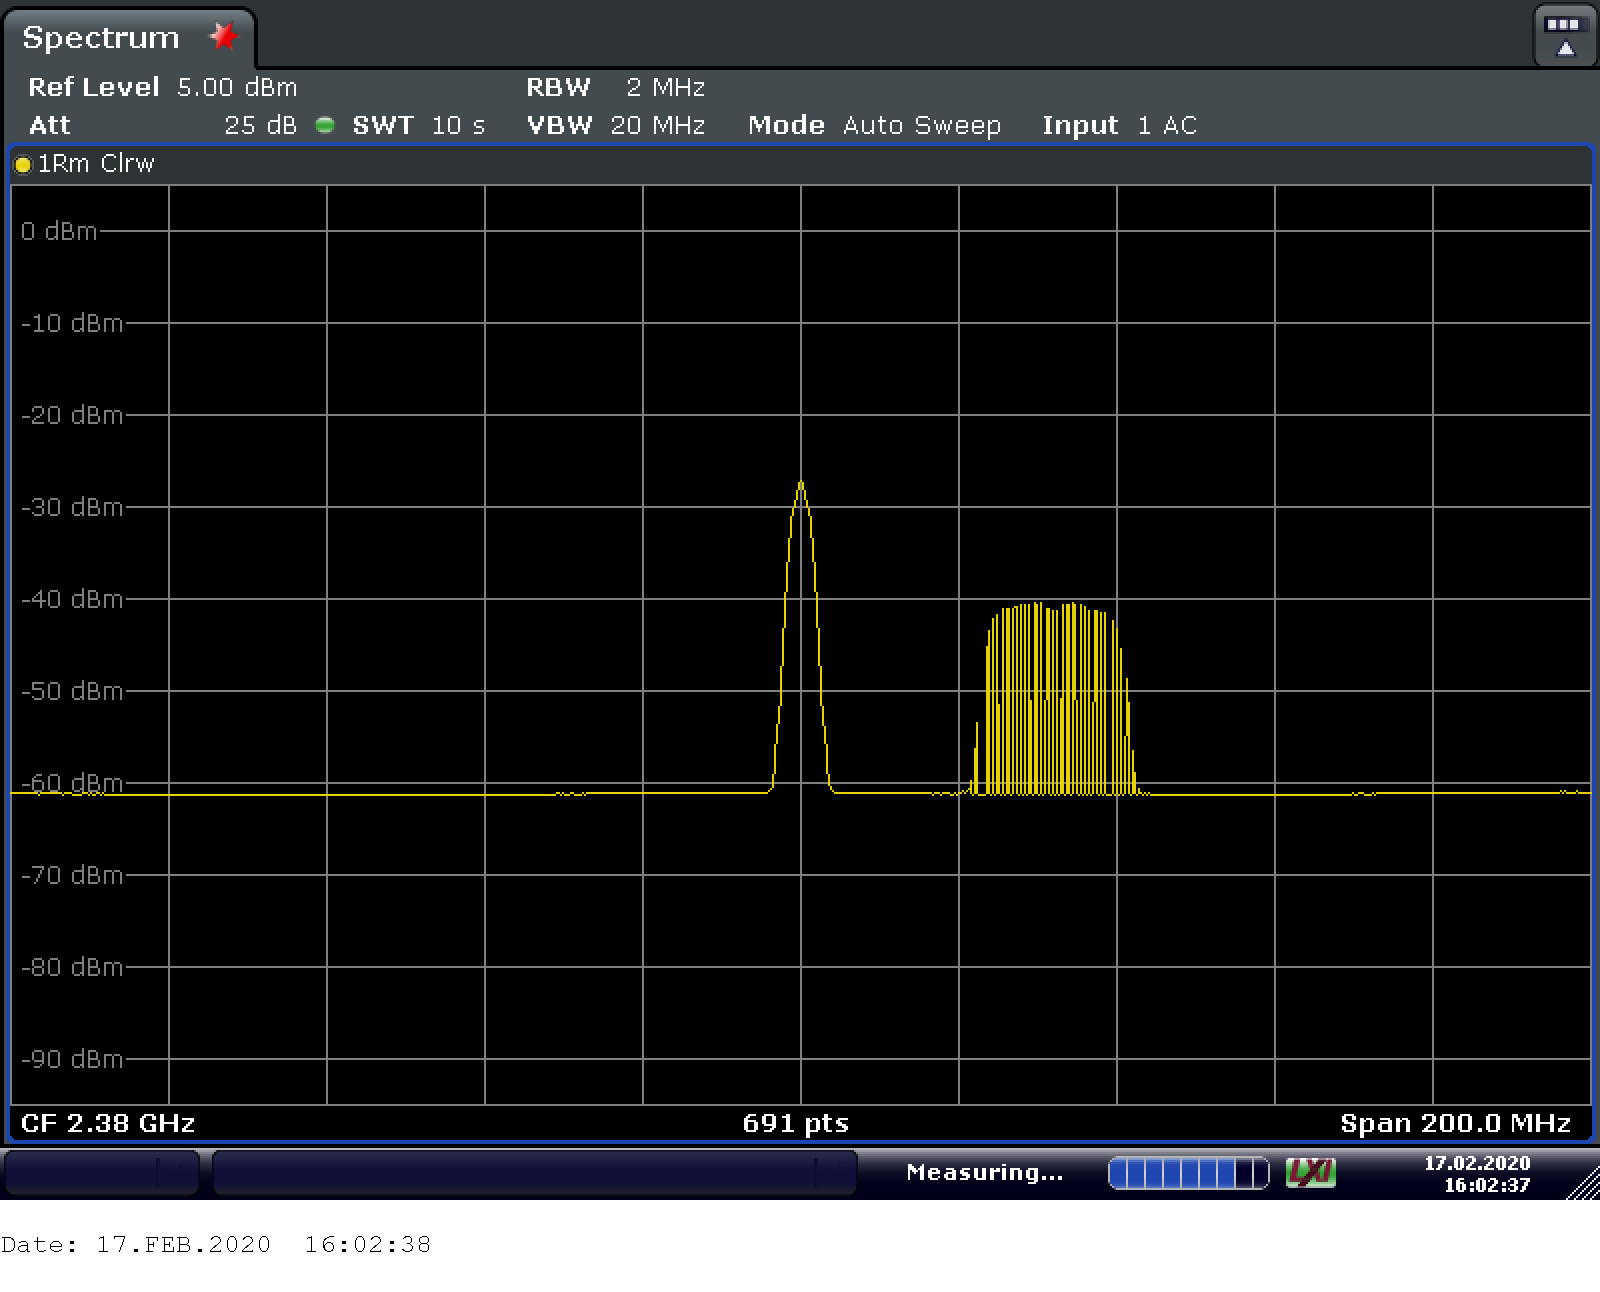
\includegraphics[scale = 0.24]{analyzer_rx.PNG}
\caption{Trace on the spectrum analyzer \acs{GUI}}
\label{fig:ax} 
\end{figure}


\section{\acf{MU}}
\acf{MU} is evaluated by running each test case (i.e. \acf{OBW}, \acf{PSD}, and Receiver Blocking) several times and then comparing the results (i.e. standard deviation and mean) of conducted and normalized measurements. Computation of \acs{MU} is done using two \acsp{DUT} (i.e. single-antenna \acs{DUT} and multi-antenna \acs{DUT}). Since the multi-antenna \acs{DUT} does not have a cable connector, we do the measurements only radiated (i.e normalized) and comparing it with conducted is not possible. \\

For the \acs{PSD} and Receiver Blocking measurement, the calculation of mean is done by converting the power level from dBm scale to linear scale because it is physically correct to use mean from the linear scale. The standard deviation is calculated by using the power values in dBm scale. 

\subsection{Single-Antenna \acs{DUT}}
This section gathers the information of \acf{MU} for each test case for both conducted and normalized type. The following reveals the results of the long-term measurements.

\subsubsection{\acf{OBW} Measurement}
The \acs{OBW} test is run 300 times for each conducted and normalized type of measurement. Figure \ref{fig:otavscond} potrays the result from the long-term measurements.

\begin{figure}[H]
\centering
\subfigure[Conducted measurement]{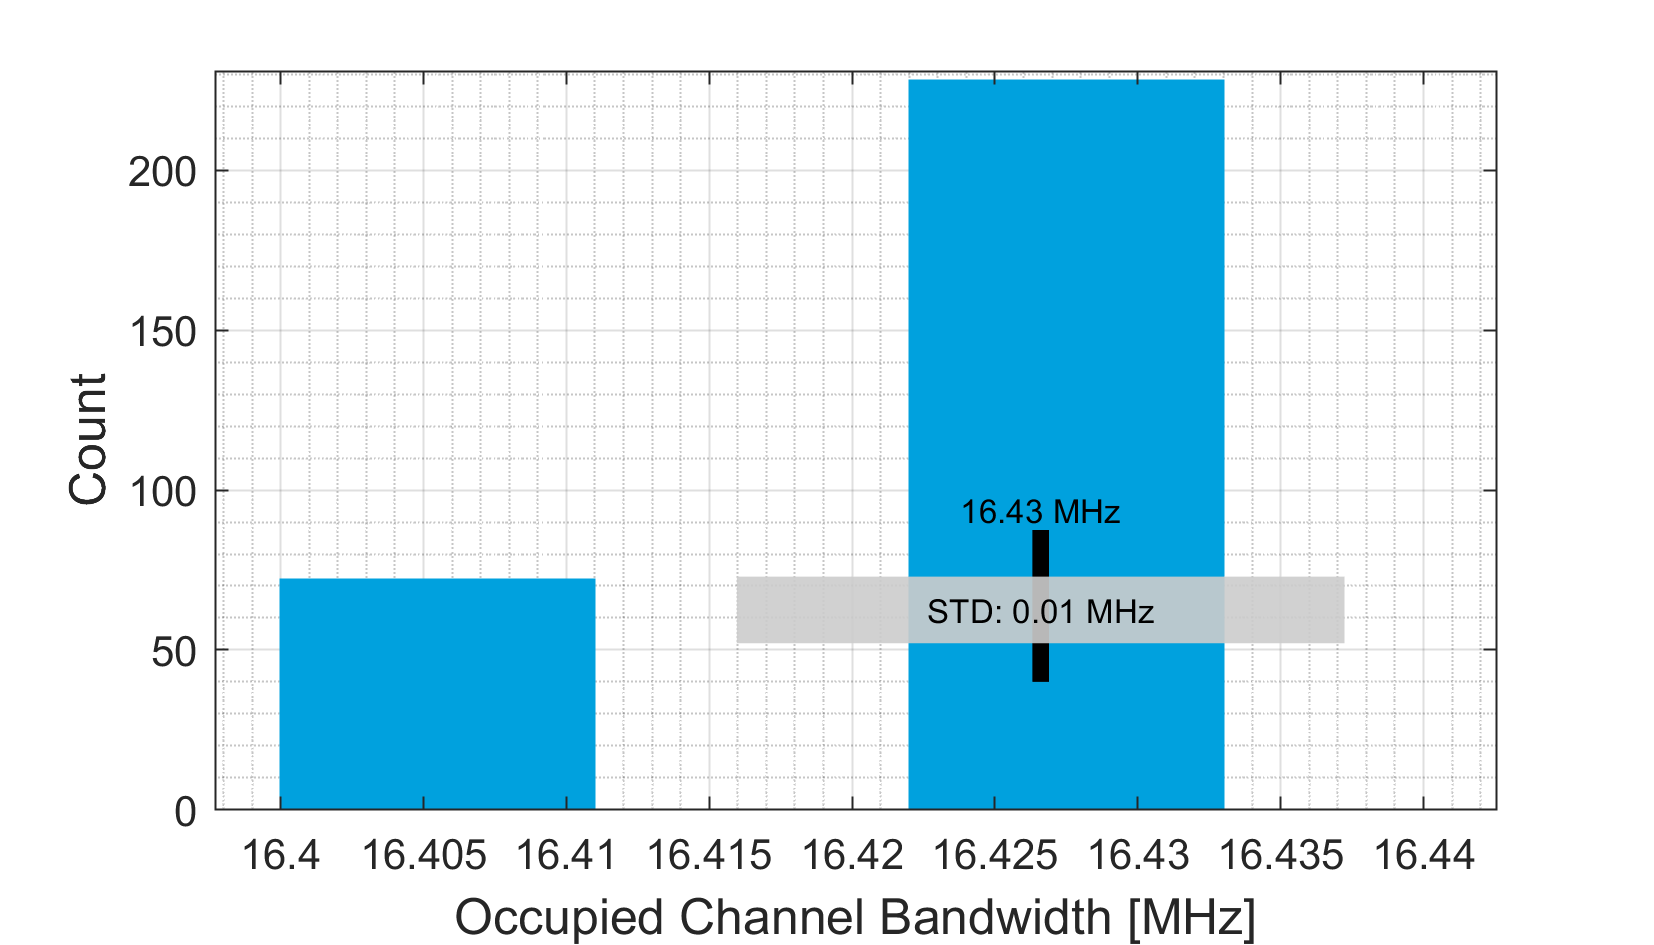
\includegraphics[scale=0.55]{bandwidth_conducted_single_300.PNG}} 
\subfigure[Normalized measurement]{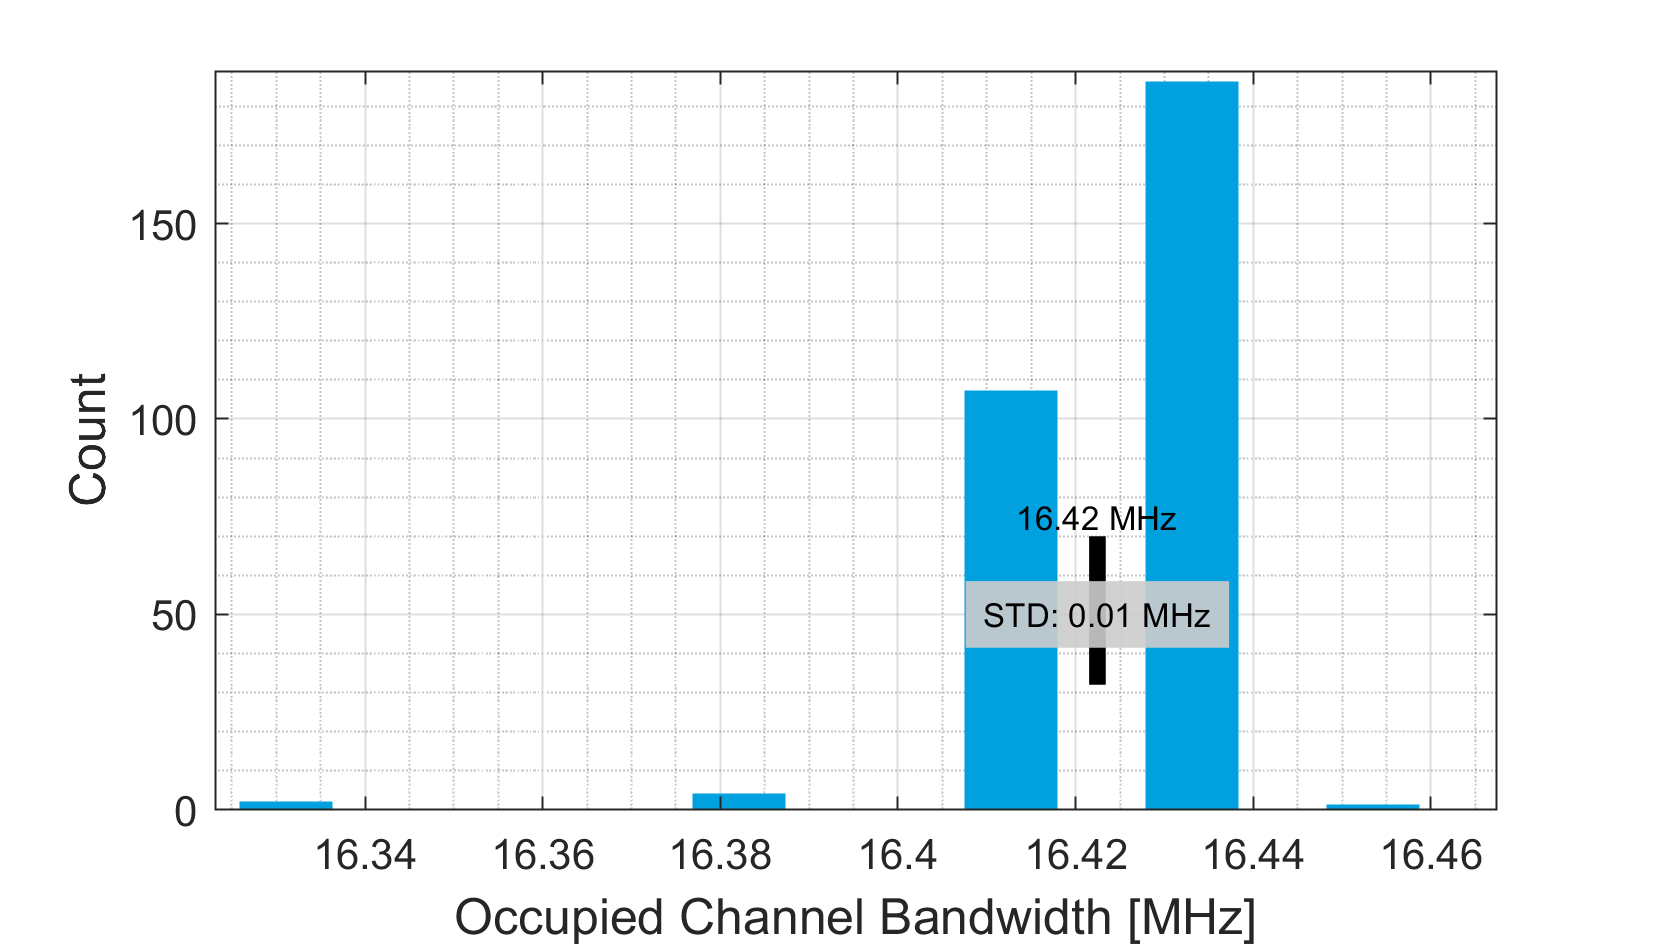
\includegraphics[scale = 0.55]{bandwidth_OTA_single_300.PNG}}  
\caption{Histogram of \acs{OBW} test-case resulting from 300 measurements }
\label{fig:otavscond} 
\end{figure}

From the plots it is clear that the \acf{MU} is almost equal in both conducted and normalized type of measurements. The table \ref{tab:tab1} arranges the results from the Figure \ref{fig:otavscond} to a tabular form. 

\begin{table}[H]
  \centering
\begin {tabular} {|c|c|c|} 
\toprule
 & \textbf{Conducted Measurement} & \textbf{Normalized Measurement} \\ 
\midrule 
\textbf{Mean} & 16.43 MHz & 16.42 MHz\\
\textbf{Standard Deviation} & 0.01 MHz & 0.01 MHz\\
\bottomrule
 \end{tabular}
  \caption{\acf{MU} results for \acs{OBW} measurement} \label{tab:tab1}
\end{table}

\subsubsection{\acf{PSD} Measurement}
The \acs{PSD} measurement is run 60 times for each conducted and normalzed type of measurement. Figure
\ref{fig:otavscond2} shows the result from the long-term measurement.
\begin{figure}[H]
\centering
\subfigure[Conducted measurement]{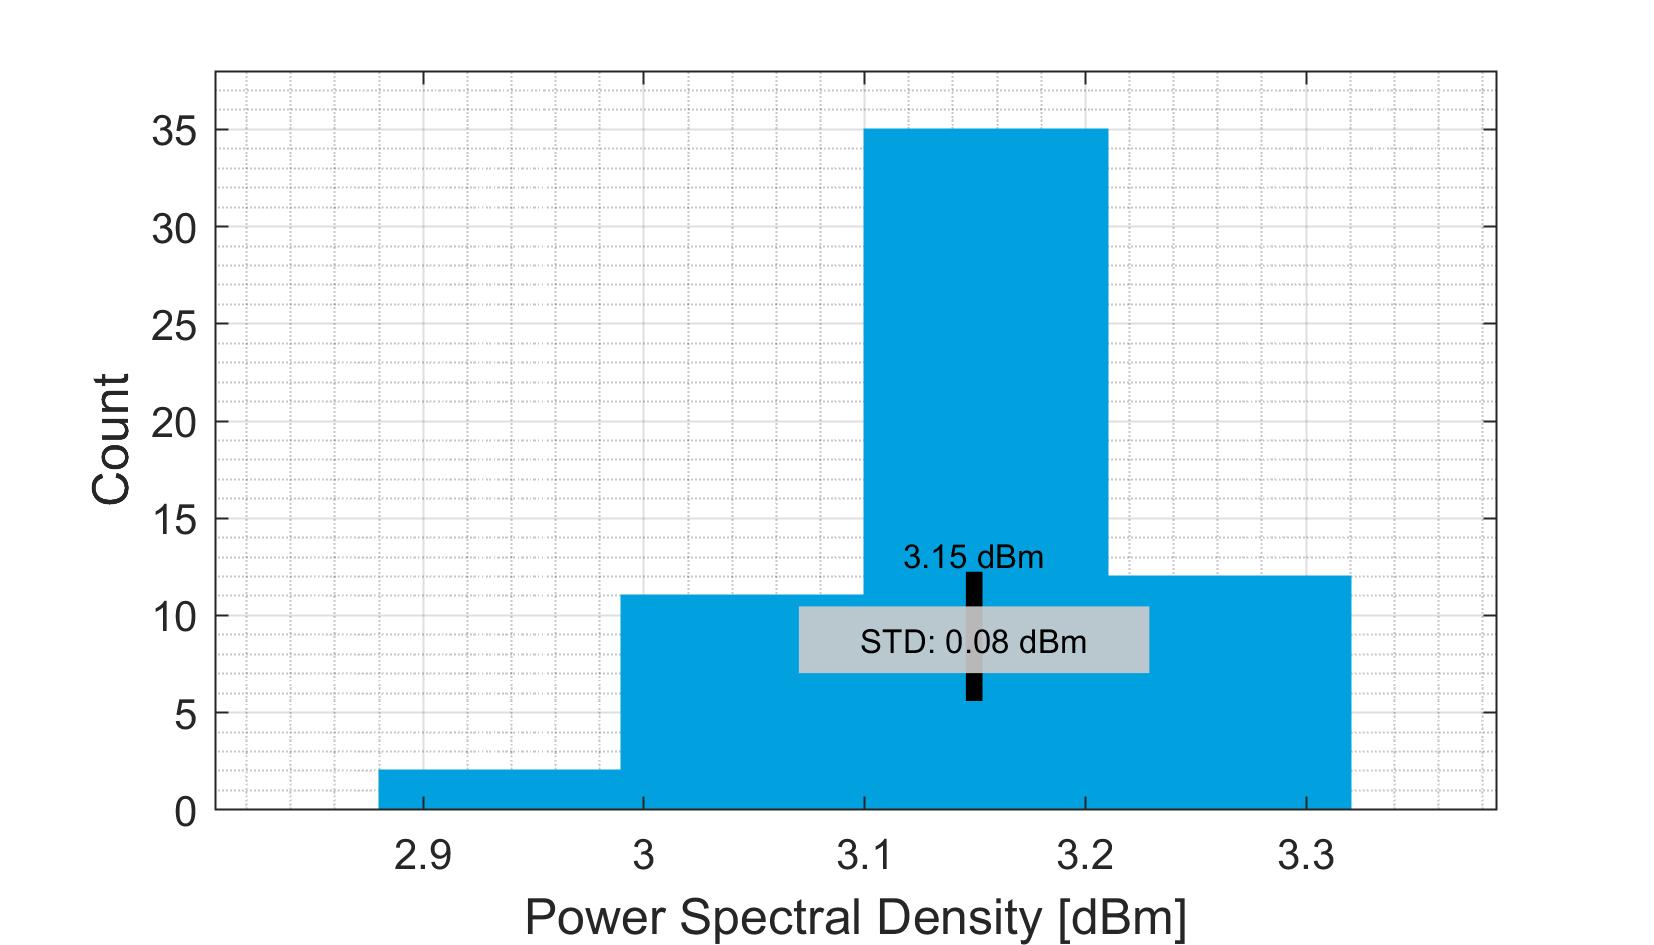
\includegraphics[scale=0.55]{PSD_conducted_single_60.PNG}}
\subfigure[Normalized measurement]{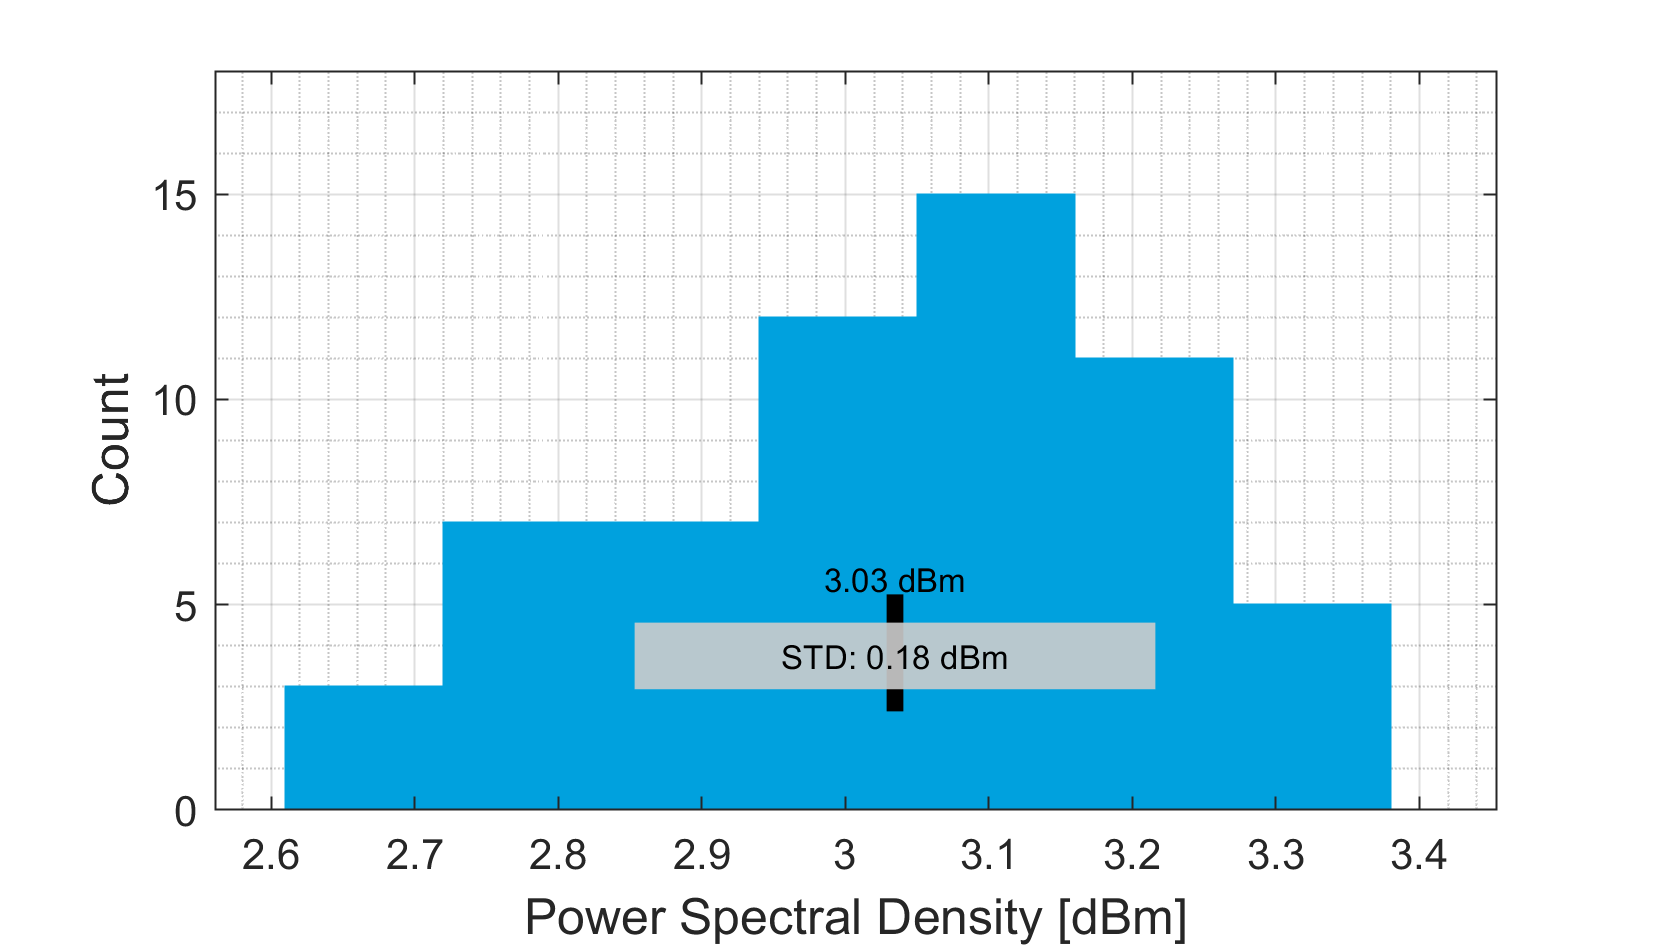
\includegraphics[scale = 0.55]{PSD_OTA_single_60.PNG}}
\caption{Histogram of \acs{PSD} test-case resulting from 60 measurements }
\label{fig:otavscond2} 
\end{figure}
It is comprehensible from the figure \ref{fig:otavscond2} as well as the table \ref{tab:tab2} that the results achieved by using conducted measurements have lower \acs{MU} compared to the ones using normalized measurements.
\begin{table}[H]
  \centering
\begin {tabular} {|c|c|c|} 
\toprule
 & \textbf{Conducted Measurement} & \textbf{Normalized Measurement} \\ 
\midrule 
\textbf{Mean} & 3.15 dBm & 3.03 dBm\\
\textbf{Standard Deviation} & 0.08 dBm & 0.18 dBm\\
\bottomrule
 \end{tabular}
  \caption{\acf{MU} results for \acs{PSD} measurement} \label{tab:tab2}
\end{table}


\subsubsection{Receiver Blocking Measurement}
The Receiver Blocking measurement is run 60 times for each conducted and normalzed type of measurement. Figure \ref{fig:otavscond3} presents the occurrence of the blocker level which results in 10\% PER at each frequency in a long-term measurement.
\begin{figure}[H]
\centering
\subfigure[Conducted measurement]{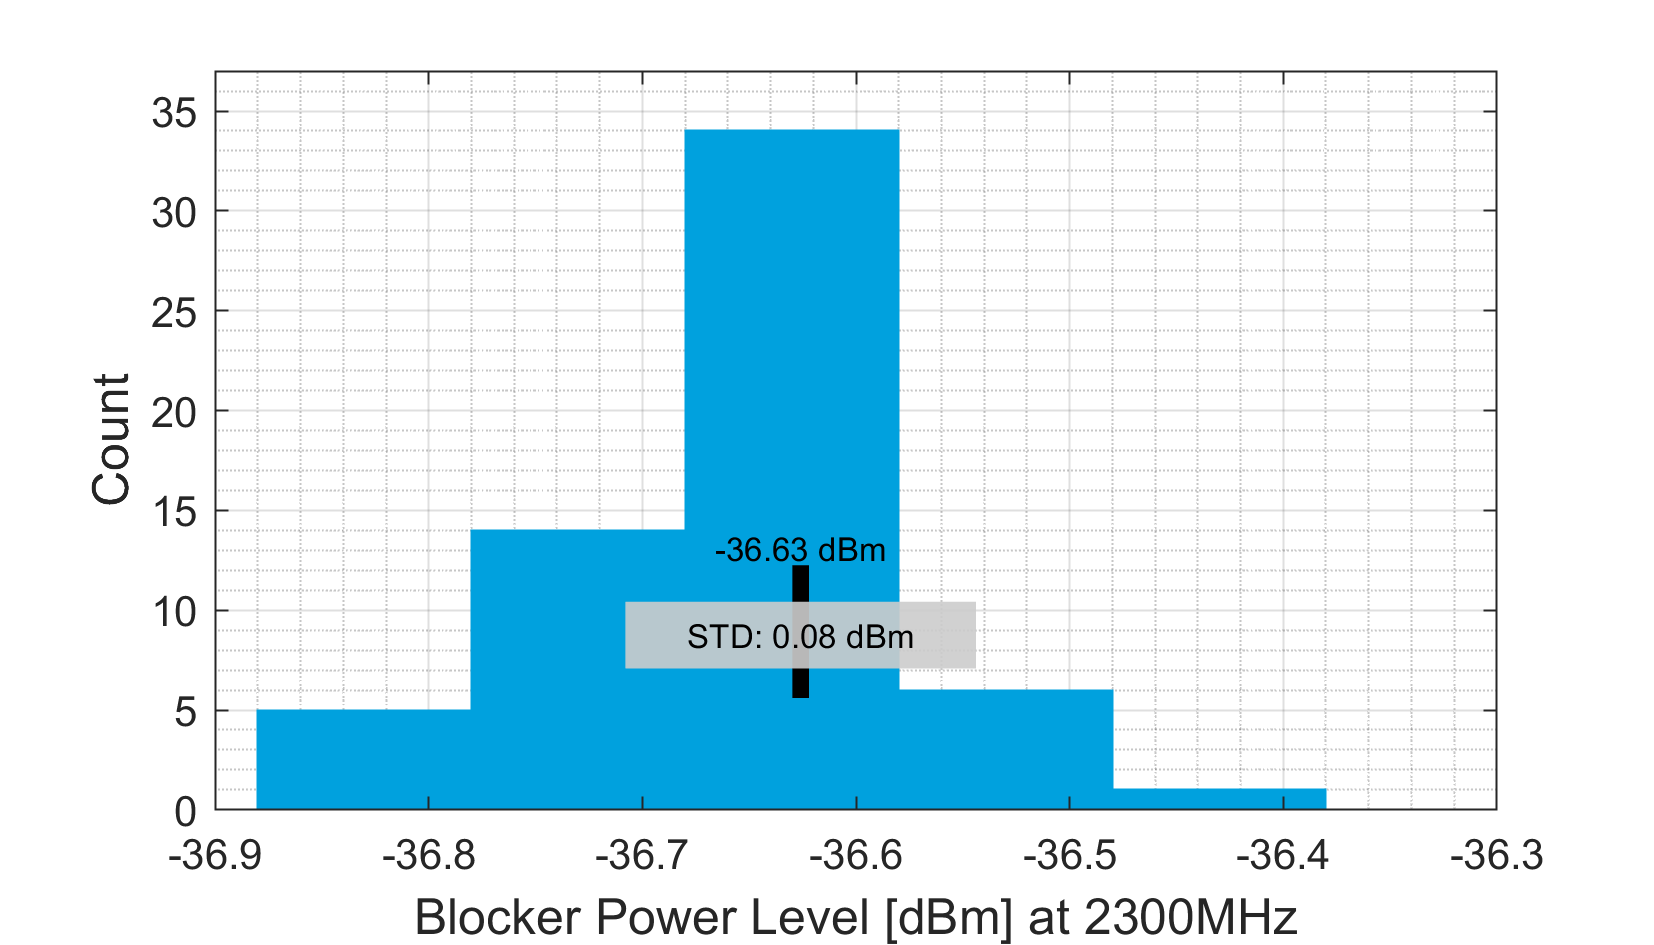
\includegraphics[scale=0.55]{RxBlocking_conducted_singleAntenna_2300_60.PNG}}
\subfigure[Normalized measurement]{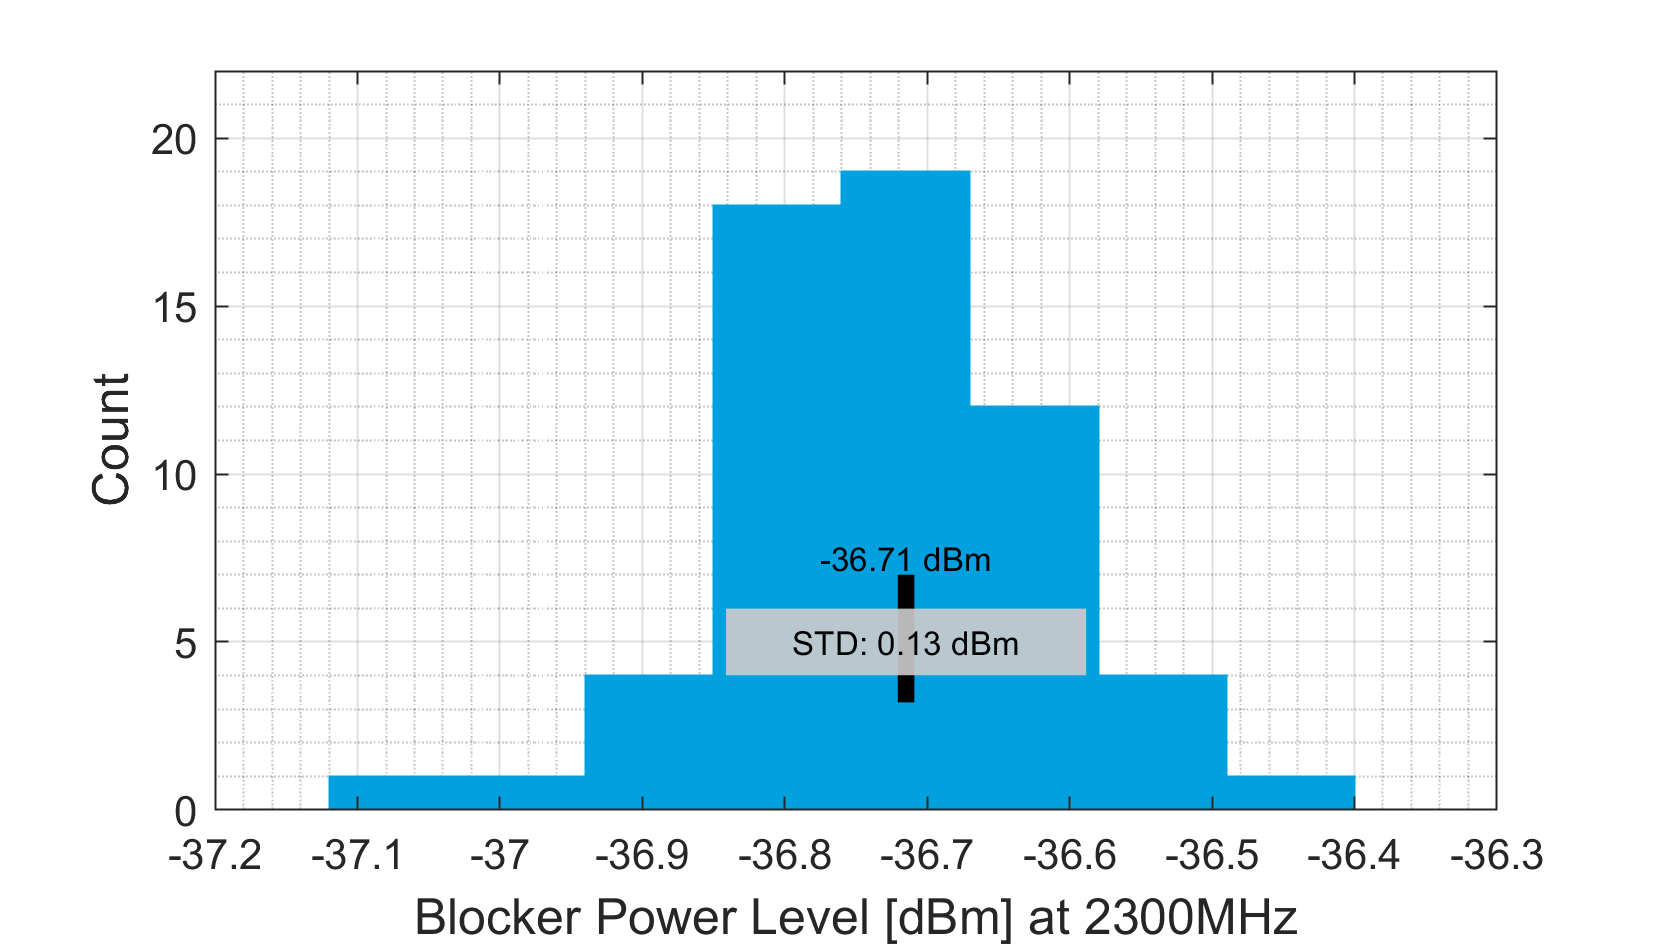
\includegraphics[scale=0.55]{RxBlocking2300.PNG}} \\
\subfigure[Conducted measurement]{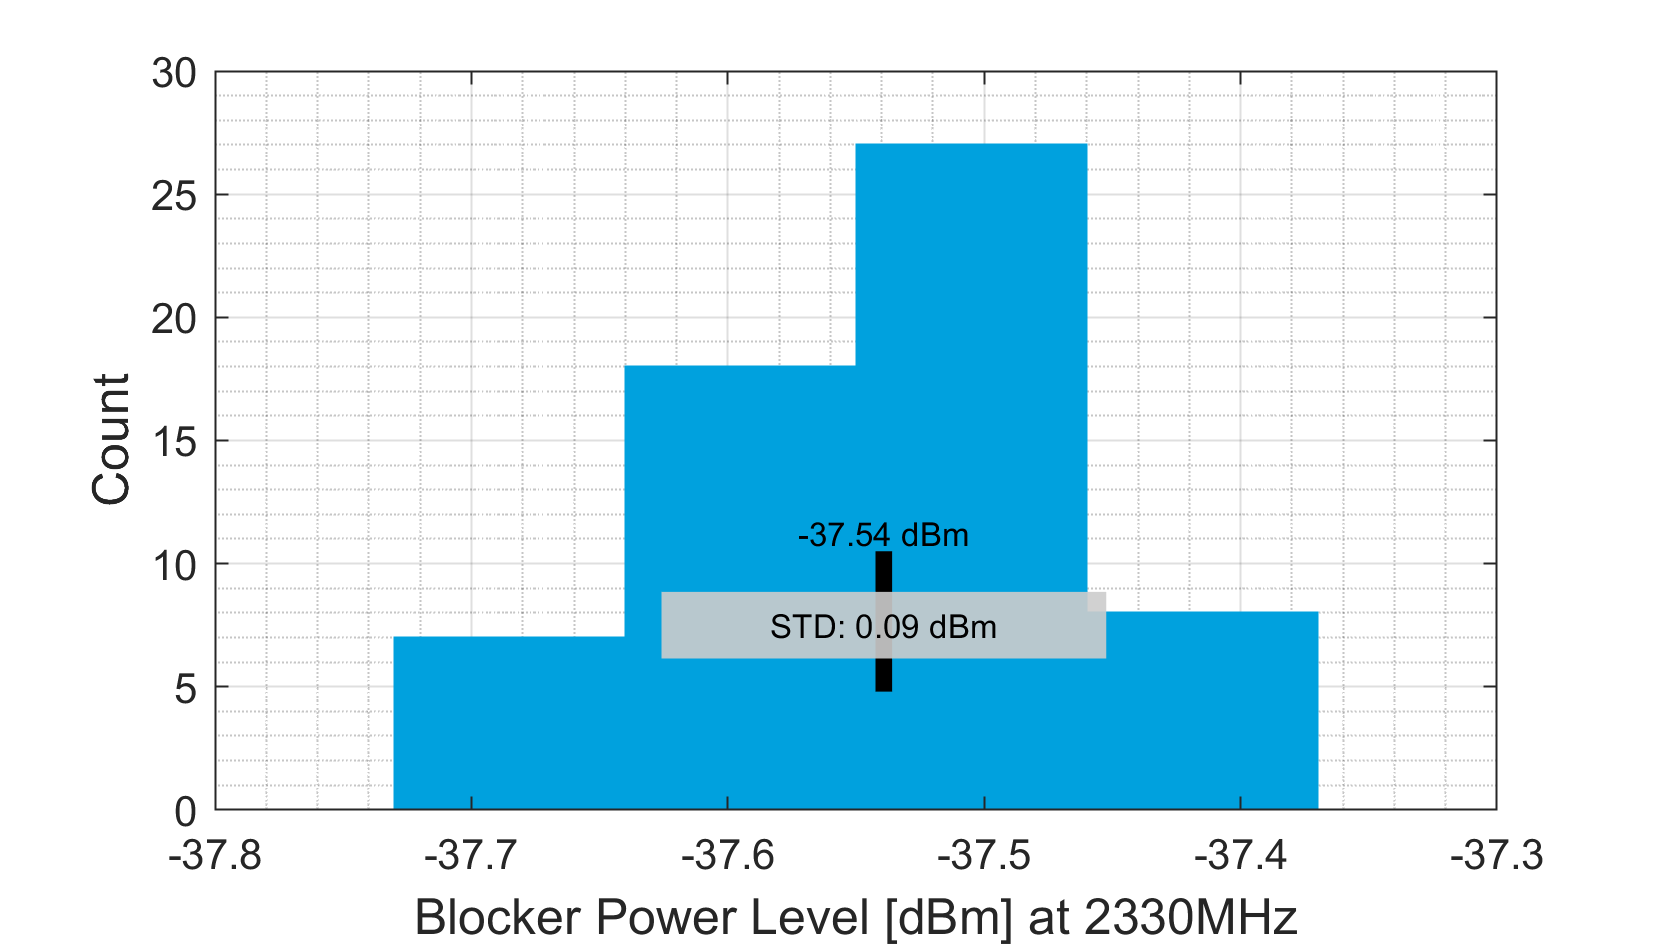
\includegraphics[scale=0.55]{RxBlocking_conducted_singleAntenna_2330.PNG}}
\subfigure[Normalized measurement]{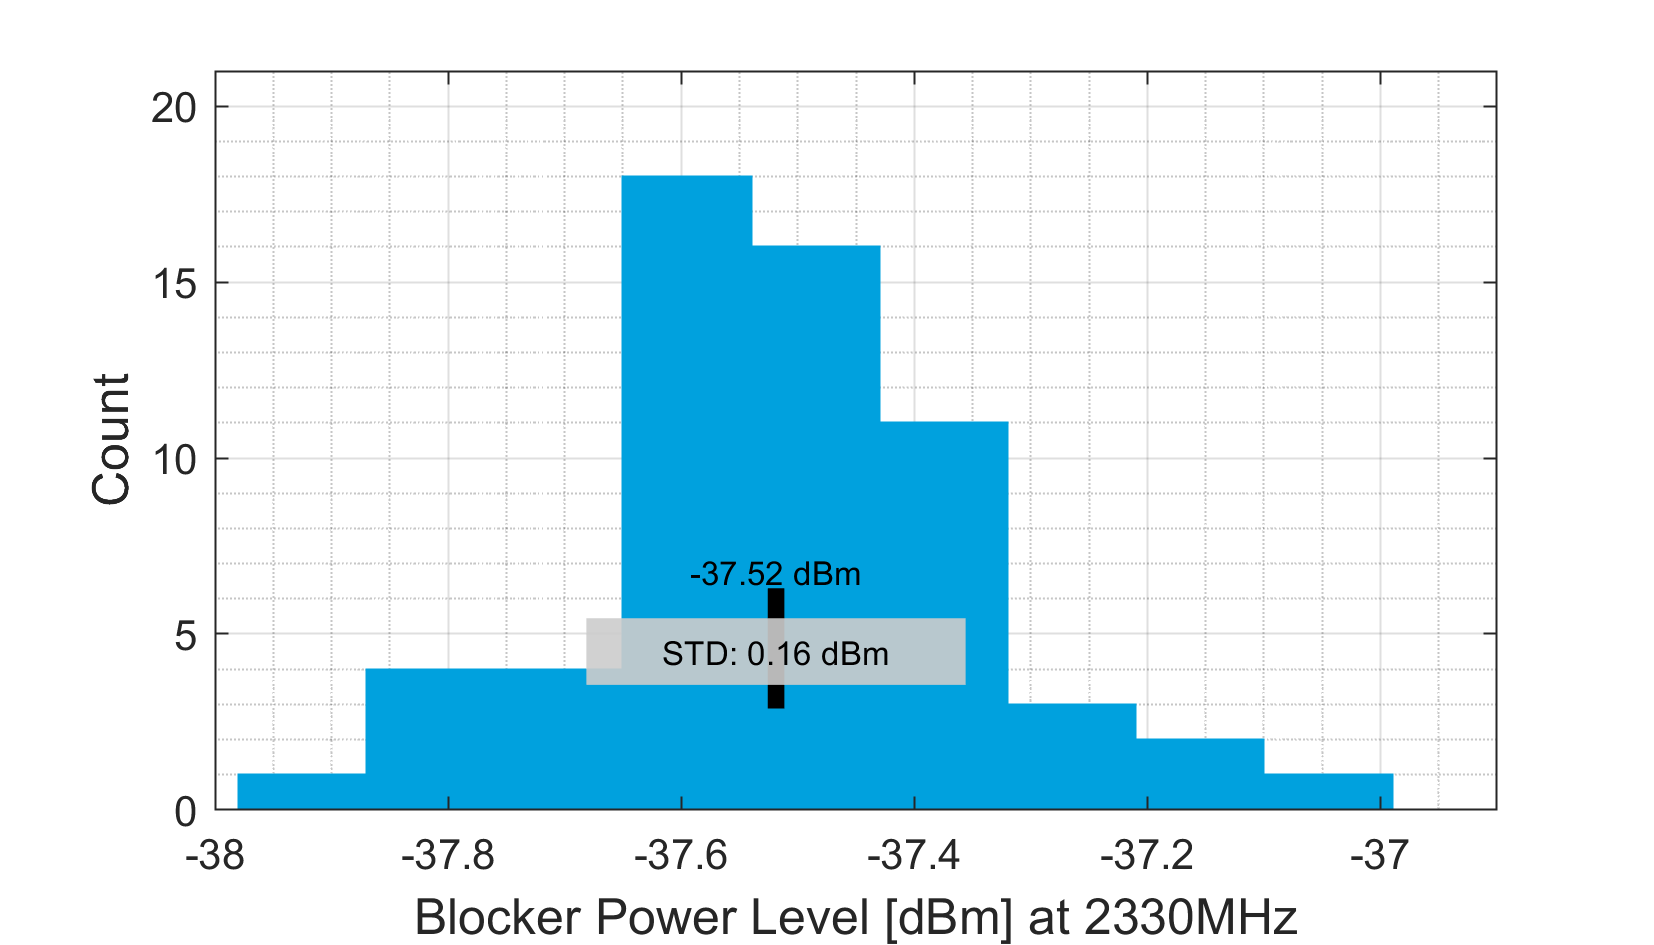
\includegraphics[scale=0.55]{RxBlocking2330.PNG}} \\
\subfigure[Conducted measurement]{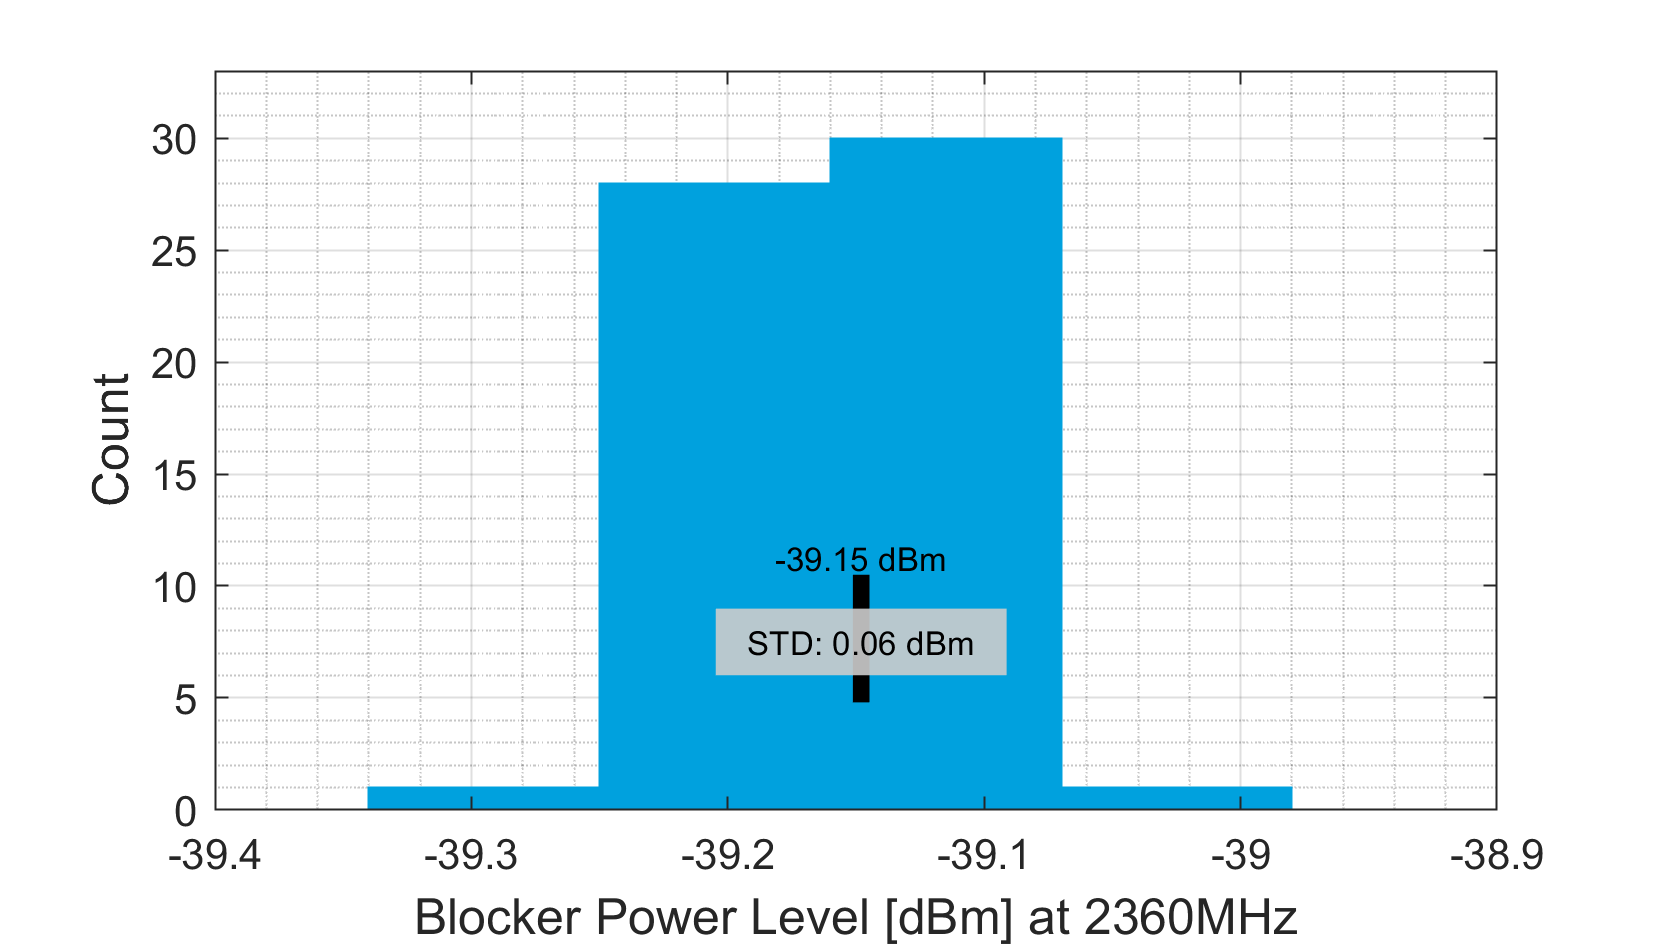
\includegraphics[scale=0.55]{RxBlocking_conducted_singleAntenna_2360.PNG}}
\subfigure[Normalized measurement]{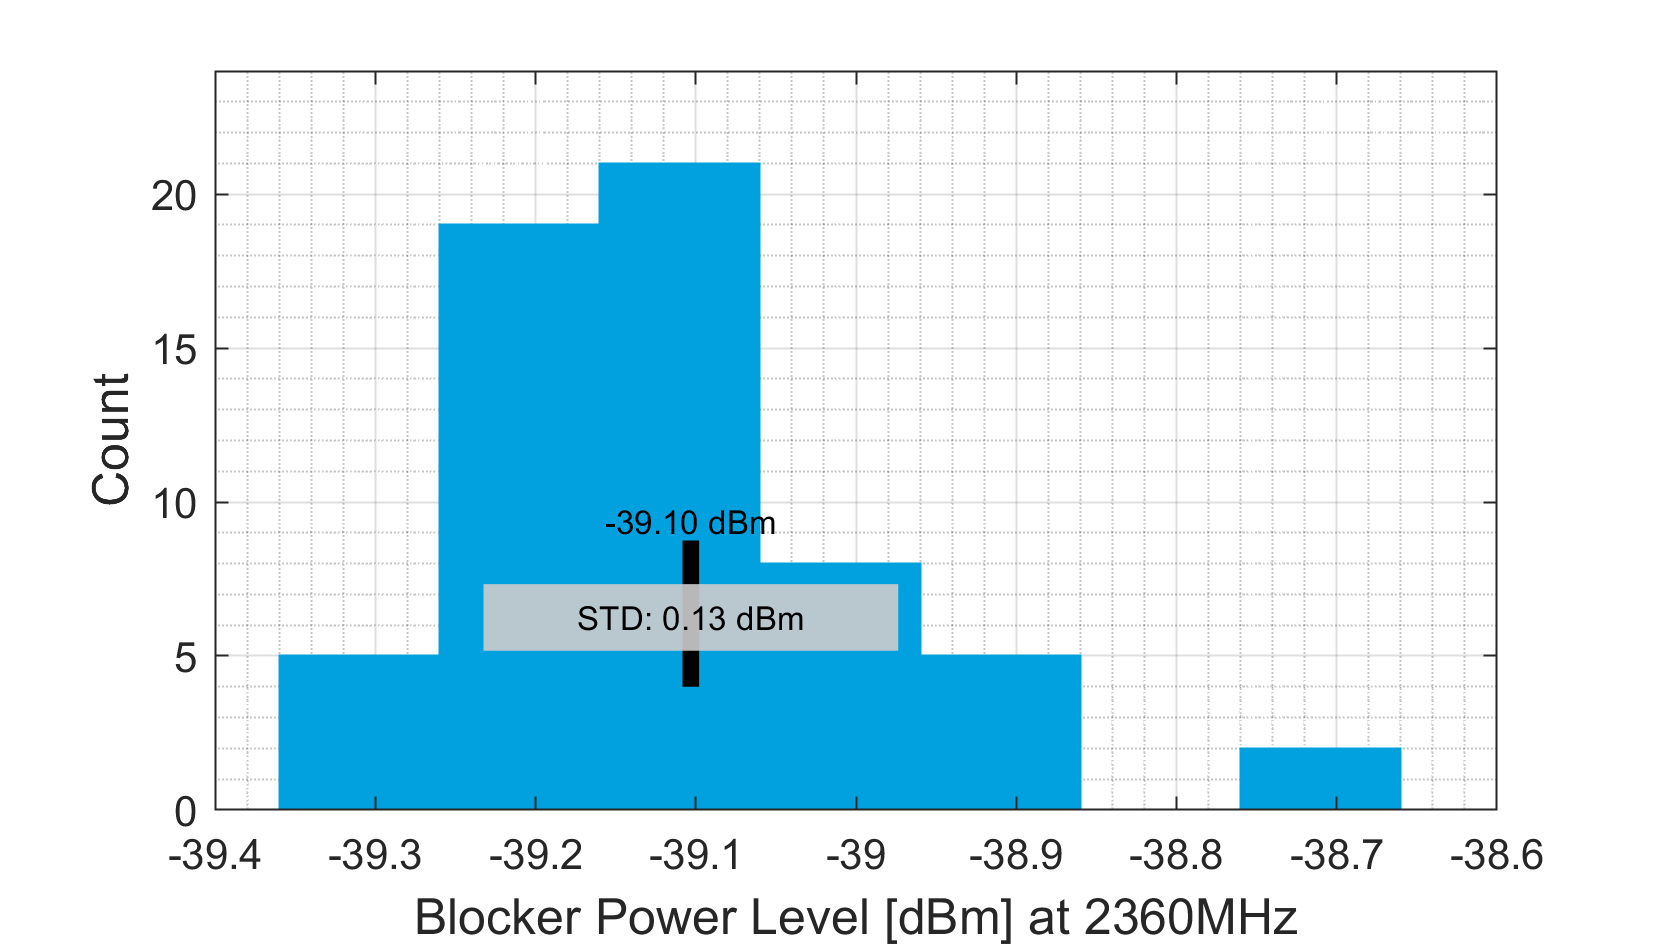
\includegraphics[scale=0.55]{RxBlocking2360.PNG}} \\
\subfigure[Conducted measurement]{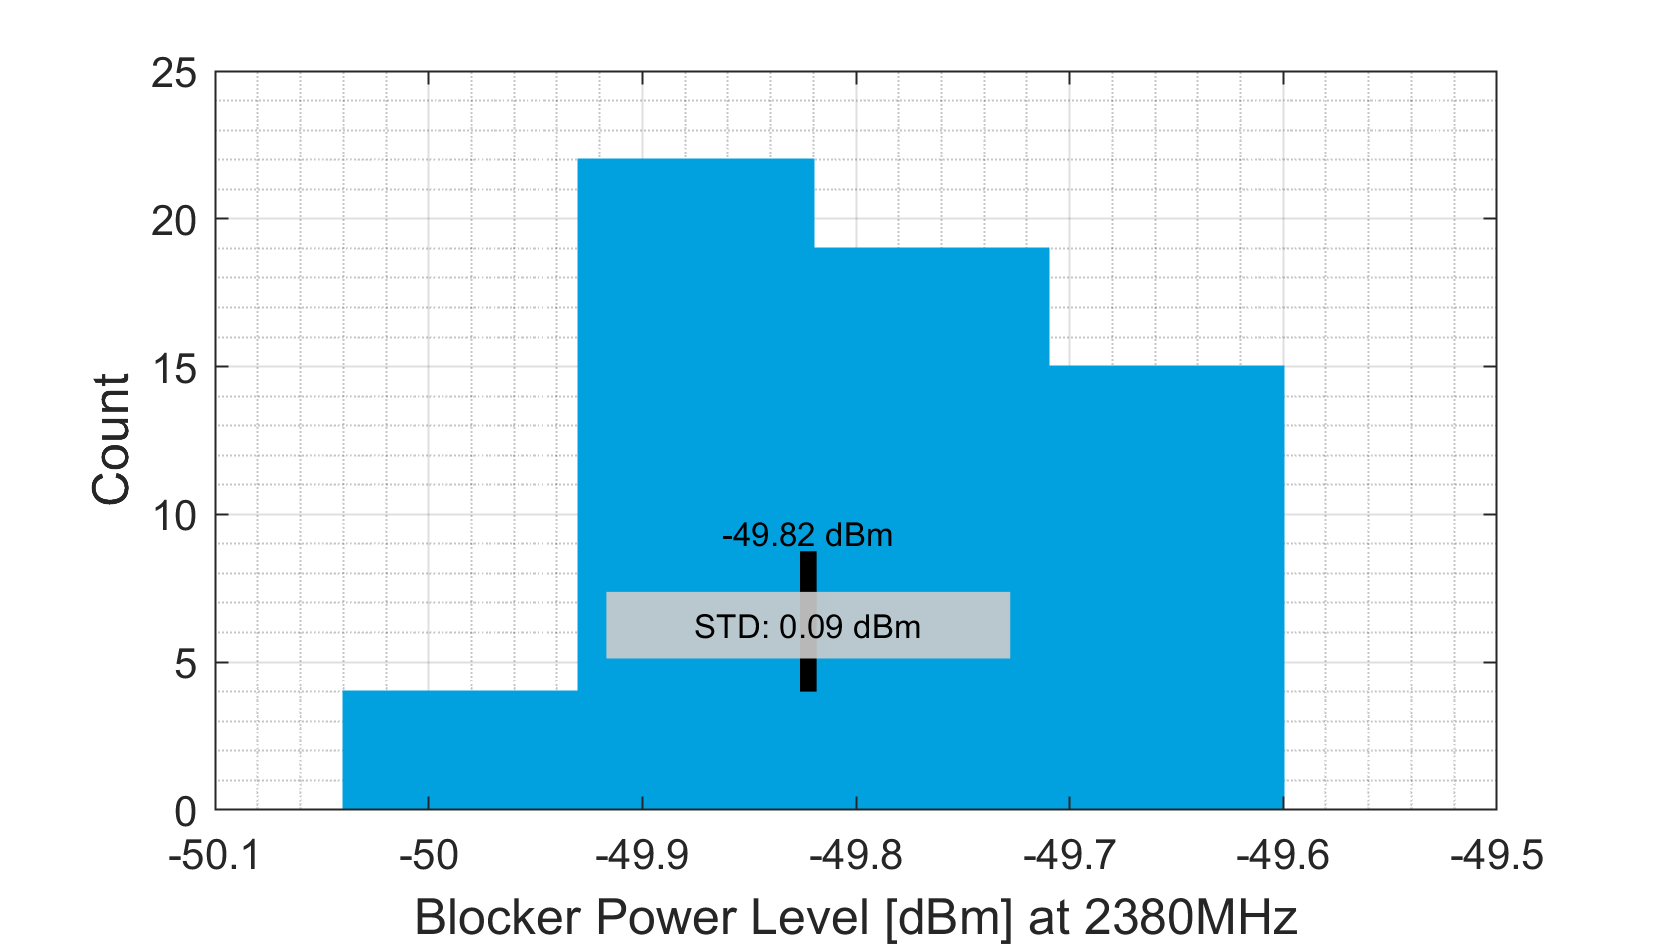
\includegraphics[scale=0.55]{RxBlocking_conducted_singleAntenna_2380.PNG}}
\subfigure[Normalized measurement]{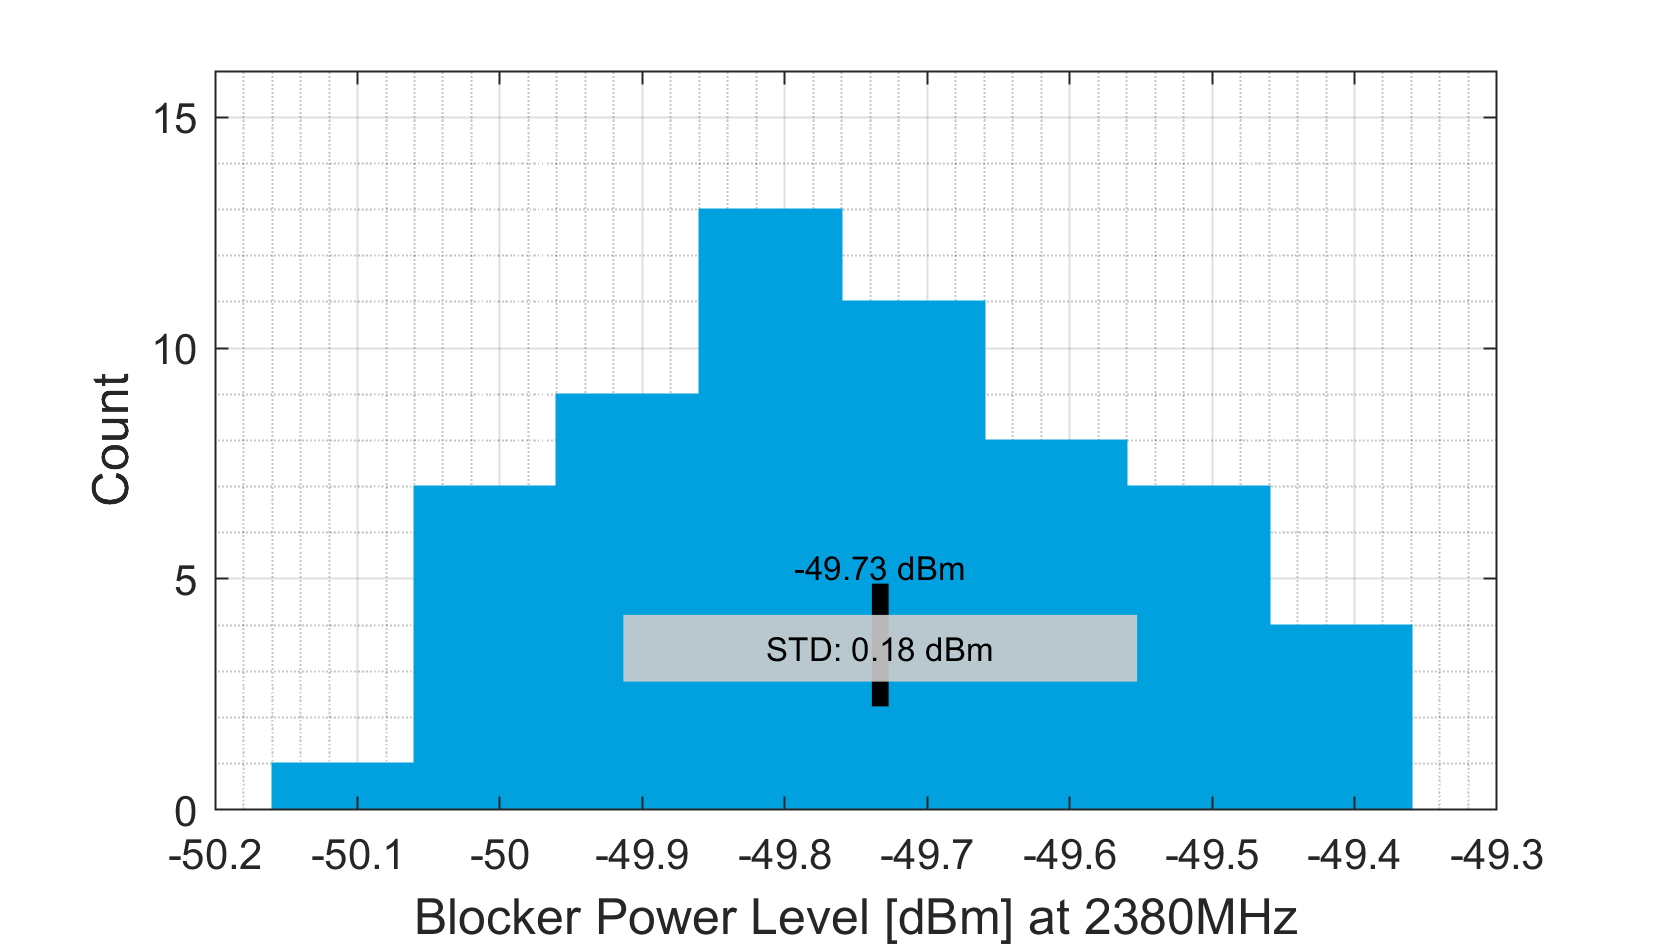
\includegraphics[scale=0.55]{RxBlocking2380.PNG}} \\
\caption{Histogram of Receiver Blocking test-case resulting from 60 measurements }
\label{fig:otavscond3} 
\end{figure}

Also in this test-case, the conducted measurement results appear to have lower \acs{MU}. In all the three test-cases, the measurement results by normalized measurements are close to the ones performed by performing the measurements in a conducted way.
\begin{table}[H]
\resizebox{\textwidth}{!}
{
        \begin{tabular}{|c|c|c|c|}\toprule
         \textbf{Blocker Frequency} & \textbf{MU Parameters} &\textbf{Conducted Measurement} & \textbf{Normalized Measurement} \\
            \midrule
            \textbf{2300 MHz} & Mean                      & -36.63 dBm & -36.71 dBm \\
                             & Standard Deviation & 0.08 dBm    & 0.13 dBm  \\
                             \midrule
            \textbf{2330 MHz} & Mean                      & -37.54 dBm & -37.52 dBm       \\
                             & Standard Deviation & 0.09 dBm    & 0.16 dBm       \\
                             \midrule
            \textbf{2360 MHz} & Mean                      & -39.15 dBm & -39.10 dBm     \\
                             & Standard Deviation & 0.06 dBm    & 0.13 dBm      \\
                             \midrule
            \textbf{2380 MHz} & Mean                      & -49.82 dBm & -49.73 dBm       \\
                             & Standard Deviation & 0.09 dBm    & 0.18 dBm \\
           \bottomrule
        \end{tabular}}
        \caption{\acf{MU} results for Receiver Blocking measurement}\label{tab:Tab3}
 \end{table} 




\subsection{Multi-Antenna \acs{DUT}}
The same three measurements are performed using multi-antenna \acs{DUT}. The measurements are run for the same number of times as the previously depicted single-antenna \acs{DUT}. Table \ref{tab:tab4} lays out the results for mean and standard deviation from the test-cases.
\begin{table}[H]
\resizebox{\textwidth}{!}
{
        \begin{tabular}{|c|c|c|c|}\toprule
         \textbf{Test-Case} & Parameters & \textbf{MU Parameters} & \textbf{Normalized Measurement} \\
            \midrule
           Receiver Blocking & 2300 MHz & Mean     & -33.03 dBm \\
                         &    & Standard Deviation & 0.14 dBm     \\

          &  2330 MHz & Mean     & -31.16 dBm       \\
                     &        & Standard Deviation & 0.12 dBm    \\

          &  2360 MHz & Mean       & -29.01 dBm    \\
                          &   & Standard Deviation & 0.13 dBm      \\
                           
          &  2380 MHz & Mean      & -35.64 dBm    \\
                       &      & Standard Deviation & 0.09 dBm     \\
                       \midrule
                      
          Occupied Channel Bandwidth & 99\% bandwidth & Mean & 16.50 MHz \\
           &  & Standard Deviation & 0.02 MHz \\
           
           \midrule
           Power Spectral Density &   maximum (mean(EIRP)) & Mean &  3.20 dBm \\
           & & Standard Deviation & 0.11 dBm \\          
           \bottomrule
        \end{tabular}}
        \caption{\acf{MU} results for measurements using Multi-Antenna \acs{DUT}}\label{tab:Tab4}
 \end{table} 

The specification sheet of this \acs{DUT} mentions that the device uses beam-forming. In-order to examine whether the \acs{DUT} performs beam-forming, a long-term power measurement to calculate the coupling loss (refer section \ref{sec:11}) is done. Measurements were performed after with random time gaps between the two measurements to investigate if the results differ due to beam-forming. The Figure \ref{fig:11} shows the result of coupling loss for 70 measurements with random time gap. 

\begin{figure}[H]
\centering
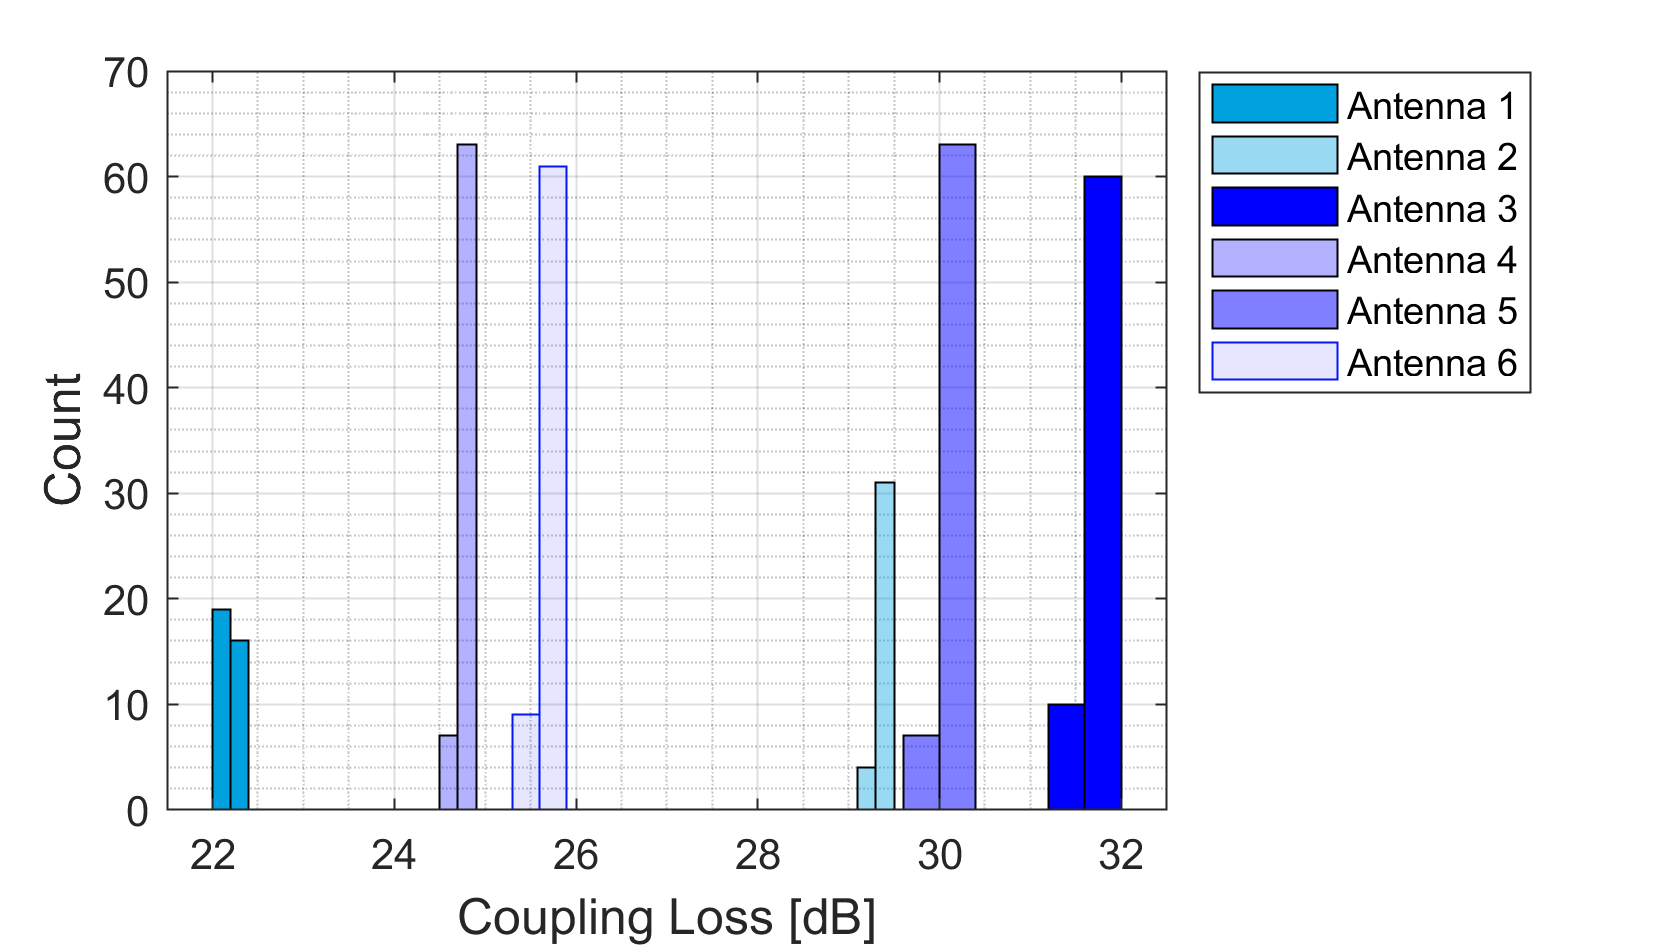
\includegraphics[scale = 0.75]{Beamforming_all_new.PNG}
\caption{Investigating beam-forming performance of the \acs{DUT}}
\label{fig:11} 
\end{figure}

Since the measurement values are almost the same, this proves that the \acs{DUT} does not perform beam-forming at 2.4 GHz.







